\label{sec_billed}

\subsection{Lokalisering af nummerplader}
\label{sec:system:lokalisering}
%\subsection{Identifikation af nummerplader}
I arbejdet med at lokalisere nummerplader, har vi valgt at arbejde med fem forskellige metoder til at udpege interesseområder i vores billeder. Det er vores tanke, at vi ved at bruge metoderne sammen kan opnå et bedre resultat end ved at bruge metoderne hver for sig. For eksempel vil et område som udpeges som værende en nummerplade af flere metoder have en høj grad af troværdighed mens det i en situation hvor metoderne alle udpeger forskellige områder vil være meget usikkert hvor nummerpladen befinder sig. I dette afsnit beskriver vi de forskellige metoder vi benytter os af, samt hvordan disse fungerer som et samlet system til lokalisering af nummerplader. I alle vores eksempler har vi brugt billedet på figur \vref{fig:typisk_billede} som inddata. Figur \vref{fig:dia_trin1} viser hvordan de fem metoder arbejder sammen om at udpege interesseområder, og hvordan der efterfølgende bliver valgt en enkelt nummerpladekandidat som bliver sendt videre i systemet. Figur \vref{fig:illu:plates_not_rotated-1} i bilag \ref{sec:illu} viser eksempler på hvordan nummerpladekandidaterne kan se ud.


\begin{figure}[htp]
\centering
\includegraphics[width=12cm]{system/illu/dia_trin1.png} 
\caption{Inddata, i form af et billede, kommer ind i systemet fra venstre. De fem metoder udpeger hver deres bud på hvor nummerpladen befinder sig og resultaterne sammenlignes. Uddata er en nummerpladekandidat.}
\label{fig:dia_trin1}
\end{figure}

%\subsubsection*{Interesseområder}
Metoderne i dette afsnit fungerer alle på den måde, at de arbejder med et binært\footnote{Et billede der kun består af farverne hvid og sort.} billede hvor områder der opfattes som interessante, det vil sige potentielle nummerplader, er markeret med farven hvid. I den bedst tænkelige, og meget urealistske, situation er nummerpladeområdet som det eneste markeret med hvidt mens resten af billedet er sort som vist i figur \vref{fig:binary_ideal}. I den realistiske situation er der mange interesseområder markeret i det binære billede som det kan ses i figur \vref{fig:binary_real}. Efter først at have beskrevet hvordan vi udvælger interesseområder, beskriver vi hvordan vi vælger mellem dem ved at vurdere i hvilket omfang de har karakteristika der er typiske for billeder af nummerplader. 

Nogle af de metoder vi bruger er baseret på materiale vi har læst, mens andre er baseret på ideer der er opstået på baggrund af vores egen analyse af nummerpladebillederne.

%SKAL DER REFERES TIL BILLEDET AF BILEN?

%\begin{figure}[htp]
%\centering
%\framebox{\includegraphics[width=5cm]{illu/B_XC33139.jpg}}
%\caption{Et billede hvor vi ønsker at lokalisere nummerpladen}
%\label{fig:input_billede}
%\end{figure}
\begin{figure}[htbp]
  \centering
  \begin{minipage}[b]{5 cm}
    \framebox{\includegraphics[width=4cm]{system/illu/binary_ideal.png}}
    \caption{Det bedst tænkelige billede af nummerpladekandidater i billedet i figur \ref{fig:typisk_billede}}
    \label{fig:binary_ideal} 
  \end{minipage}
  \begin{minipage}[b]{5 cm}
    \framebox{\includegraphics[width=4cm]{system/illu/binary_real.png}}  
  \caption{Et mere realistisk eksempel på nummerpladekandidater for billedet i figur \ref{fig:typisk_billede}.}
  \label{fig:binary_real} 
  \end{minipage}
\end{figure}

\begin{comment}
\begin{figure}[htp]
\centering
\includegraphics[width=5cm]{system/illu/binary_ideal.png} 
\caption{Det bedst tænkelige billede af nummerpladekandidater i billedet i figur \ref{fig:input_billede}}
\label{fig:binary_ideal}
\end{figure}
SKAL DER VÆRE ET BILLEDE DER VISER SITUATIONEN FØR DER SORTERES FRA?
\begin{figure}[htp]
\centering
\includegraphics[width=5cm]{system/illu/binary_real.png} 
\caption{Et mere realistisk eksempel på nummerpladekandidater for billedet i figur \ref{fig:input_billede}.}
\label{fig:binary_real}
\end{figure}

\end{comment}


\subsubsection{Metode: Områder domineret af lyse gråtoner}
\label{sec:DetectSameness}
I denne metode forsøger vi at finde nummerpladen i et billede ved at lede efter områder der domineres af lyse gråtoner i et farvebillede. Vi håber at et af de markerede interesseområder vil være nummerpladen, da dens baggrund består af lyse gråtoner. I et farvebillede vil det sige, at området vil være domineret af pixels hvor de tre farvekanaler, rød, grøn og blå har intensitetsværdier der ligger forholdsvis tæt på hinanden. Som et eksempel på det modsatte, vil en helt rød pixel have maksimal intensitet i den røde farvekanal mens intensiteterne i den grønne og blå farvekanal vil være minimale. I dette tilfælde er der altså tale om en meget skæv fordeling af intensitetsværdierne mellem de tre farvekanaler. Et eksempel på en jævn fordeling af intensitetsværdierne er en middelgrå pixel. Den vil have en middel intensitetsværdi i alle tre farvekanaler. Denne metode er inspireret af metoder beskrevet af \cite{ron} og \cite{nijhuis}, der dog begge forsøger at lokalisere nummerplader med en mere karakteristisk, gul baggrund.

For at markere interesseområder udregner vi en gennemsnitsværdi, $M$ for hver pixel i farvebilledet ved at summere værdierne for hver af de tre farvekanaler og dividere med tre. Hvis alle tre kanaler har en værdi der ligger tæt på gennemsnitsværdien, og denne samtidig er høj, det vil sige at pixelen er lys, markeres den indeværende pixels position i det binære billede der viser interesseområderne med hvidt. Figur \ref{fig:DetectSameness-binary} viser et eksempel på intereseområder markeret med denne metode. 

\begin{comment}
Hvis $X$ er en nedre grænseværdi for de intensiteter vi opfatter som lyse. $Y$ er en værdi der bestemmer hvor stor afstand der må være mellem intensiteterne i de tre farvekanaler og $I_{ij}$ er pixels i et farvebillede hvis nummerplade vi ønsker at finde, er pixels i det binære billede $B_{ij}$ defineret som:
\begin{equation}
B_{ij} = 
\begin{Bmatrix}
1 & \text{Hvis } (R(I_{ij})+G(I_{ij})+B(I_{ij})/3) > X\\
 & R(I_{ij}) > mean - Y & < Y + mean\\
0 & \delta
\end{Bmatrix}
\end{equation}

HVORDAN SKRIVES DETTE I LATEX?


\end{comment}

\begin{comment}
For hver pixel $x$ i et farvebillede, hvor vi ønsker at finde nummerpladen, udregnes værdien for samme pixel $x_{b}$ i det binære billede således:

\begin{equation}
x_{b} = 
\begin{Bmatrix}
1 & \text{Hvis } M > L\\
 & M-D > R(x) < M+D\\
  & M-D > G(x) < M+D\\
   & M-D > B(x) < M+D\\
0 & \text{ellers..}
\end{Bmatrix}
\end{equation}


hvor $M = ((R(x)+G(x)+B(x))/3)$ og $R(x)$, $G(x)$ og $B(x)$ er intensitetsværdierne for henholdsvis den røde, den grønne og den blå farvekanal i pixelen $x$, mens $L$ er den nedre grænse for middelværdien og $D$ er den maksimale afstand fra værdien i de tre farvekanaler til $M$.

\end{comment}


\begin{figure}[htbp]
  \centering
  \begin{minipage}[b]{5 cm}
    \framebox{\includegraphics[width=4cm]{illu/B_XC33139.jpg}}
  \end{minipage}
  \begin{minipage}[b]{5 cm}
    \framebox{\includegraphics[width=4cm]{system/illu/DetectSameness-binary.png}}  
  \end{minipage}
  \caption{Det binære billede til højre viser de interesseområder metoden markerer når inddata er billedet til venstre.}
  \label{fig:DetectSameness-binary}
\end{figure}



\subsubsection{Metode: Områder med høj kontrast}
\label{sec:DetectContrastAvg}
Vi forventer at et område med en nummerplade vil indeholde områder med høj kontrast på grund af de mange skarpe kanter mellem de mørke tegn og den lyse baggrund. Ved at lave billedet om til gråtoner og derefter opfatte intensiteterne i billedet som højder i et landskab, kan vi beskrive hældninger i landskabet med såkaldte gradienter. Metoden beskrevet i dette afsnit er baseret på systemet beskrevet i \cite{shapiro}.

Gradienter beskriver hældningen i en pixel som en todimensionel vektor. Et område med en blød overgang i intensitet fra sort til hvid, har korte gradienter der alle peger den samme vej for alle pixels i området, mens et område med en brat overgang fra sort til hvid (høj kontrast) vil resultere i lange gradienter, der peger mod det sorte område. Figur \vref{fig:gradienter} viser to simple eksempler på intensitetslandskaber og de tilhørende gradienter.

\begin{figure}[htp]
\centering
\includegraphics[width=10cm]{system/illu/gradienter.png} 
\caption{Illustration af konceptet gradienter. Pilene viser hældninger i intensitetslandskabet. Da der er tale om glidende overgange fra hvid til sort, har pilene alle samme længde. Hvis der havde været områder med pludselige skift i intensitet, ville gradienterne i disse områder have været de længste. Illustrationen er fra \cite{wiki_gradienter}.}
\label{fig:gradienter}
\end{figure}

Efter at have udregnet billedets gradienter som vist i figur \vref{fig:DetectContrastAvg-grads}, kan vi udregne deres vinkler. Vi vælger at lave et nyt billede der viser gradienter med en vinkel på mellem $0^{\circ}$ og $30^{\circ}$ mellem sig selv og en vandret linie. Et eksempel på et sådant billede er vist i figur \vref{fig:DetectContrastAvg-hgrads}. Grunden til at vi kun tager disse ``liggende'' gradienter med, er at vi på den måde undgår at markere eventuelt vandrette kanter i billedet der måtte forbinde nummerpladen med bilens lygter eller andet. Vores håb er, at der er nok lodrette kanter i nummerpladeområdet til at det stadig bliver markeret på billedet der viser de vandrette gradienter. For eksempel ville en plade med to forekomster af bogstavet \textbf{I} og seks forekomster af tallet \textbf{1} være meget synlig på vores gradientbillede mens en nummerplade hvor begge bogstaver er et \textbf{O} og alle seks cifre er tallet \textbf{0} være mindre synlig på grund af det lavere antal lodrette kanter og deraf følgende lave antal vandrette gradienter.
% Input image & gradients
\begin{figure}[htbp]
  \centering
  \begin{minipage}[b]{5 cm}
    \framebox{\includegraphics[width=4cm]{illu/example_car_gray.jpg}}
  \end{minipage}
  \begin{minipage}[b]{5 cm}
    \framebox{\includegraphics[width=4cm]{system/illu/DetectContrastAvg-grads.png}}  
  \end{minipage}
  \caption{Billedet til højre viser gradienterne i billedet til venstre. Området med nummerpladen er tydeligt markeret på grund af de store kontraster i området.}
  \label{fig:DetectContrastAvg-grads}
  \end{figure}

% Horizontal gradients
\begin{figure}[htp]
  \centering
  \framebox{\includegraphics[width=10cm]{system/illu/DetectContrastAvg-hgrads.png}}
  \caption{Gradienterne fra figur \vref{fig:DetectContrastAvg-grads} med vinkler mellem $0^\circ$ og $30^\circ$ grader. Bemærk at de vandrette linier der er synlige over og under nummerpladen i figur \ref{fig:DetectContrastAvg-grads} ikke er synlige i denn figur.}
  \label{fig:DetectContrastAvg-hgrads}  
\end{figure}


Før vi laver det binære billede med nummerpladekandidater, forsøger vi at gøre nummerpladeområdet til en sammenhængende figur ved at udtvære (\textit{eng.: to blur}) billedet med et filter, der giver hver pixel en intensitet svarende til middelværdien for dens nærområde. Da vi primært er interesserede i at forbinde pixels der ligger ved siden af hinanden (tegnene i nummerpladen) og ønsker at undgå at nummerpladeområdet bliver forbundet med områder der ligger tæt på dens over- og underkant, definerer vi nærområdet som et liggende rektangel. Resultatet bliver et sammenhængende område med en højde svarende til højden på tegnene i nummerpladen og en bredde der er noget længere end nummerpladens bredde. Et eksempel er vist i figur \vref{fig:DetectContrastAvg-blurredGrads}. 

% Blured horizontal gradients
\begin{figure}[htp]
  \centering
  \framebox{\includegraphics[width=10cm]{system/illu/DetectContrastAvg-blurredGrads.png}}
  \caption{De markerede områder i nummerpladen i figur \vref{fig:DetectContrastAvg-hgrads} forbindes ved at give hver pixel en intensitet der er proportional med gennemsnittet i nærområdet.}
  \label{fig:DetectContrastAvg-blurredGrads}  
\end{figure}


Som det sidste trin laver vi et binært billede med interesseområder som vist i figur \vref{fig:DetectContrastAvg-binary}. Vi bruger en forholdsvis lav grænseværdi når vi laver dette billede. Det vil sige, vi udover de meget lyse områder også opfatter forholdsvis mørkegrå områder som intereseområder da vi ønsker at nummerpladen skal blive et sammenhængende område i det binære billede.

%Binary image
\begin{figure}[htp]
  \centering
  \framebox{\includegraphics[width=10cm]{system/illu/DetectContrastAvg-binary.png}}  
  \caption{Det binære billede med nummerpladekandidater der er afledt af billedet i figur \vref{fig:DetectContrastAvg-blurredGrads}.}
  \label{fig:DetectContrastAvg-binary}
\end{figure}

\subsubsection{Metode: Frekvensanalyse}
\label{sec:DetectPlateness}
Ved at analysere svingningen mellem lyse og mørke intensiteter i de nummerplader der indgår i vores træningsæt, forsøger vi med denne metode at lokalisere nummerplader ved at markere de områder der har en frekvens der ligger tæt på den målte middelfrekvens for nummerpladeområder som observeret i vores træningsæt.  For hver pixel i billedet analyserer vi frekvensen af en linie der begynder et givent antal pixels før den indeværende pixel og slutter det samme antal pixels efter. Vi undersøger hvor mange gange intensiteten stiger op over og falder ned under middelværdien for området. Det er dette tal vi bruger som et udtryk for frekvensen i området. Dette princip er illustreret på figur \vref{fig:DetectPlateness-frekvensanalyse}. Metoden er inspireret af \cite{kwas} der også arbejder med frekvensanalyse for at lokalisere nummerplader. Figur \vref{fig:DetectPlateness-binary} viser et eksempel på den type binære billeder frekvensanalysen resulterer i.

% FREKVENS
\begin{figure}[htp]
  \centering
  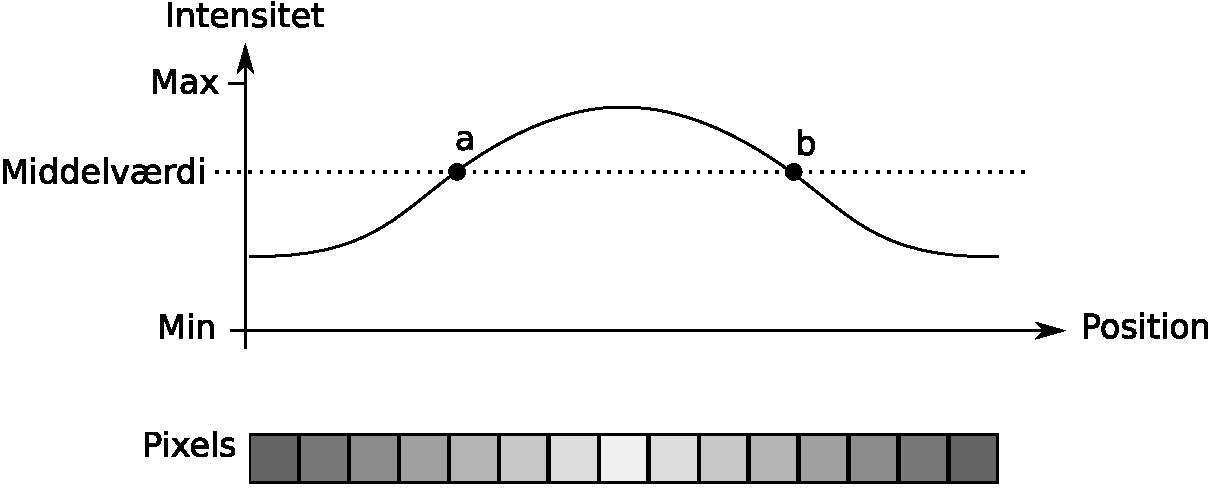
\includegraphics[width=12cm]{system/illu/frekvensanalyse.pdf}  
  \caption{Illustration af frekvensanalyse: For den række pixels der er vist nederst i figuren ønsker vi at analysere frekvensen. Ved at måle intensiteterne i rækken af pixels får vi kurven og middelværdien der er angivet i koordinatsystemet. Kurven der repræsenterer intensiteterne i rækken af pixels krydser middelværdien to gange i punkterne \textbf{a} og \textbf{b}. Antallet af skæringer med middelværdien bruger vi som et udtryk for frekvensen i området. I dette tilfælde er antallet 2.}
  \label{fig:DetectPlateness-frekvensanalyse}
\end{figure}

%Binary image
\begin{figure}[htp]
  \centering
  \framebox{\includegraphics[width=10cm]{system/illu/DetectPlateness-binary.png}}  
  \caption{Interesseområder som udpeget ved frekvensanalyse.}
  \label{fig:DetectPlateness-binary}
\end{figure}

\subsubsection{Metode: Maksimer lokal kontrast}
\label{sec:DetectContrastStretch}
Ideen bag denne metode er, at vi ved at dele billedet op i små blokke og uafhængigt af intensiteterne i resten af billedet maksimere kontrasten i disse små områder, kan lave et binært billede hvor nummerpladen er et af få sammenhængende områder.

Vi maksimerer kontrasten for hver blok med såkaldt \textit{Contrast streching} som illustreret på figur \vref{fig:DetectPlateness-contrast_stretch}. Da spredningen af intensiteter i de små udsnit af billedet oftest vil være forholdsvis lille, kan vi øge kontrasten i området ved at strække intensiteterne så de udnytter hele spektret på 256 intensitetsværdier. På denne måde bliver de lyseste pixels i blokken helt hvide  mens de mørkeste bliver helt sorte. Figur \vref{fig:DetectCStretch-illu1} viser hvordan vi ved at strække intensiteterne deler et område forestillende en blød overgang fra sort til hvid over i to forskellige områder der hver har intensitetsværdier i hele spektret. En nummerplade vil derimod fortsat være en sammenhængende figur efter intensiteterne er blevet strakt, da de lyseste områder, baggrunden, i nummerpladeblokkene fortsat vil støde op til de lyseste områder i de nummerpladeblokke der ligger ved siden af. Dette forhold er illustreret i figur \vref{fig:DetectCStretch-illu2}.


\begin{figure}[htp]
  \centering
  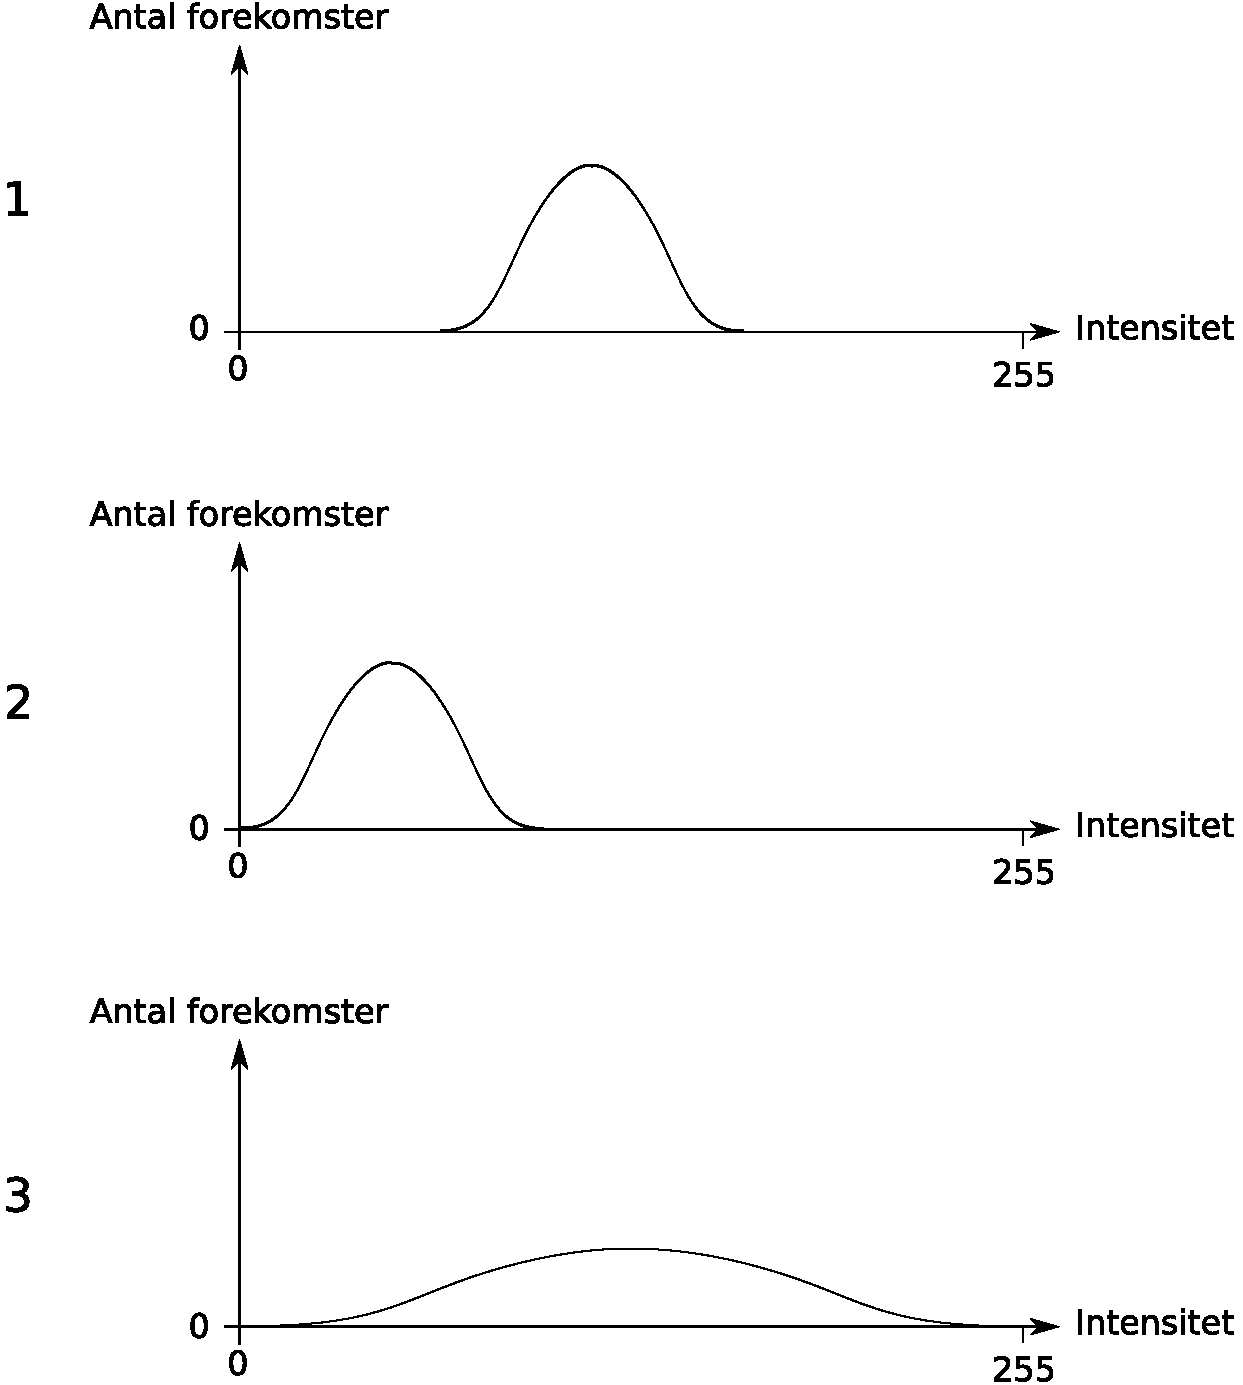
\includegraphics[width=12cm]{system/illu/contrast_stretch.pdf} 
  \caption{Forstærkelse af kontrast: For at forbedre kontrasten i et billede kan man strække intensiteterne så hele intensitetsområdet udnyttes. Figur 1 ovenfor viser antal forekomster  af intensiteter for et billede der ikke udnytter hele intensitetsområdet der går fra 0 til 255. Intensiteterne i billedet ligger alle i et ret smalt område. Vi gør alle intensiteter i billedet så meget mindre, at den mindste bliver 0 som illustreret i figur 2. Til sidst strækker vi intensiteterne så billedet udnytter alle intensiteter fra 0 til 255 som vist i figur 3. Den højeste intensitet i billedet er nu 255 og den laveste er 0.}
  \label{fig:DetectPlateness-contrast_stretch}
\end{figure}


% Illu af contrast strech
\begin{figure}[htbp]
  \centering
  \begin{minipage}[b]{5 cm}
    \framebox{\includegraphics[width=4cm]{system/illu/DetectCStretch-illu1_1.png}}
  \end{minipage}
  \begin{minipage}[b]{5 cm}
    \framebox{\includegraphics[width=4cm]{system/illu/DetectCStretch-illu1_2.png}}  
  \end{minipage}
  \caption{Billedet til højre viser resultatet af at dele billedet til venstre op i to kvadratiske blokke og strække deres intensiteter. I hver blok bliver de mørkeste toner helt sorte, og de lyseste helt hvide når intensiteterne strækkes.}
  \label{fig:DetectCStretch-illu1}
\end{figure}

% Illu af contrast strech på plade
\begin{figure}[htbp]
  \centering
  \begin{minipage}[b]{5 cm}
    \framebox{\includegraphics[width=4cm]{system/illu/DetectCStretch-illu2_1.png}}
  \end{minipage}
  \begin{minipage}[b]{5 cm}
    \framebox{\includegraphics[width=4cm]{system/illu/DetectCStretch-illu2_2.png}}  
  \end{minipage}
  \caption{Den underbelyste nummerplade til venstre deles op i to kvadratiske blokke, og intensiteterne i dem strækkes uafhængigt af hinanden. Resultatet til højre viser, at hele nummerpladen stadig er ét sammenhængende lyst område i modsætning til eksemplet i figur \vref{fig:DetectCStretch-illu1} hvor billedet bliver delt.}
  \label{fig:DetectCStretch-illu2}
\end{figure}

Med denne metode får vi det binære billede af interesseområder der er vist i figur \ref{fig:DetectCStretch-binary}.

%Binary image
\begin{figure}[htp]
  \centering
  \framebox{\includegraphics[width=10cm]{system/illu/DetectCStretch-binary.png}}  
  \caption{Det binære billede af interesseområder skabt af metoden der maksimerer lokal kontrast. Bemærk, at nummerpladen er et fritstående sammenhængende område.}
  \label{fig:DetectCStretch-binary}
\end{figure}

\subsubsection{Metode: Kvantifisering}
Med denne metode forsøger vi at lokalisere nummerplader ved at sætte antallet af gråtoner i vores inddatabillede ned fra 256 til 7. Med færre mulige intensitetsværdier vil billedet indeholde større sammenhængende områder der repræsenterer de områder i originalbilledet hvor intensiteterne ligger forholdsvis tæt på hinanden. Det er vores forventning at et af disse områder er nummerpladen.

Som det første trin i denne metode, kører vi et filter der giver en pixel den maksimale intensitet fra dens nærområde. Vi forventer at dette vil udviske tegnene på nummerpladen og efterlade et lyst rektangel i billedet der hvor nummerpladen findes. Formen på vores filter er et liggende rektangel, da vi vil forsøge at undgå at nummerpladen forbindes med lyse områder der ligger over og under nummerpladen. Et eksempel på resultatet af at anvende dette filter er vist i figur \vref{fig:DetectQuant-filteredImage}. 

%BILLEDET SKAL OPDATERES DA METODEN ER BLEVET ÆNDRET EN LILLE SMULE.
% Filtered image
\begin{figure}[htp]
  \centering
  \framebox{\includegraphics[width=10cm]{system/illu/DetectQuant-filteredImage.png}}
  \caption{Resultatet af at køre et filter der giver hver pixel samme intensitet som den maksimale intensitet i nærområdet.}
  \label{fig:DetectQuant-filteredImage}  
\end{figure}

Som næste trin sætter vi antallet af intensiteter i det filtrerede billede ned. Det giver os større sammenhængende områder med samme intensitet som vist i figur \vref{fig:DetectQuant-quantImage}. På baggrund af dette billede danner vi et binært billede der viser vores interesseområder. Et eksempel er vist i figur \vref{fig:DetectQuant-binary}.

% Quant image
\begin{figure}[htp]
  \centering
  \framebox{\includegraphics[width=10cm]{system/illu/DetectQuant-quantImage.png}}
  \caption{Resultatet af at sætte antallet af intensitetet i billedet i figur \vref{fig:DetectQuant-filteredImage} ned til syv.}
  \label{fig:DetectQuant-quantImage}  
\end{figure}

% Quant binary image
\begin{figure}[htp]
  \centering
  \framebox{\includegraphics[width=10cm]{system/illu/DetectQuant-binary.png}}
  \caption{Interesseområde valgt på baggrund af billedet i figur \vref{fig:DetectQuant-quantImage}}
  \label{fig:DetectQuant-binary}  
\end{figure}


\subsubsection{Analyse af interesseområder}
\label{sec:BinImgCleanup}
I de binære billeder der viser interesseområder, skal vi forsøge at udvælge de områder der mest sandsynligt er nummerplader. Vi begynder denne udvælgelsesproces med, at frasortere de områder vi mener at kunne udelukke som værende nummerplader. Vi sletter interesseområder med følgende karateristika:

\paragraph{1. Området er meget lille eller meget stort:}
Områdets højde og/eller bredde er meget lille eller meget stor i forhold til de nummerplader vi har observeret i træningssættet.

\paragraph{2. Området har et afvigende forhold mellem bredde/højde:}
Området har et bredde/højde forhold der ligger meget langt fra en nummerplades bredde/højdeforhold. For eksempel områder hvis højde er større en bredden. 

\paragraph{3. Området har lav densitet}
Området har få markerede pixels i forhold til det rektangel det udspænder. For eksempel vil et interesseområde med form som en enkelt skrå streg have en meget lav densitet.

Figurene \ref{fig:DetectSameness-cleanup} til \ref{fig:DetectQuant-cleanup} viser frasorteringen anvendt på de binære billeder med interesseområder som vi brugte som eksempler i beskrivelsen af de forskellige metoder til lokalisering af nummerplader. 

% SAMENESS
\begin{figure}[htbp]
  \centering
  \begin{minipage}[b]{5 cm}
    \framebox{\includegraphics[width=4cm]{system/illu/DetectSameness-binary.png}}
  \end{minipage}
  \begin{minipage}[b]{5 cm}
    \framebox{\includegraphics[width=4cm]{system/illu/DetectSameness-cleaned.png}}  
  \end{minipage}
  \caption{Frasortering af interesseområder udvalgt af metoden der markerer områder domineret af lyse gråtoner i farvebilleder}
  \label{fig:DetectSameness-cleanup}
\end{figure}

% CONTRAST AVG
\begin{figure}[htbp]
  \centering
  \begin{minipage}[b]{5 cm}
    \framebox{\includegraphics[width=4cm]{system/illu/DetectContrastAvg-binary.png}}
  \end{minipage}
  \begin{minipage}[b]{5 cm}
    \framebox{\includegraphics[width=4cm]{system/illu/DetectContrastAvg-cleaned.png}}  
  \end{minipage}
  \caption{Frasortering af interesseområder udvalgt af metoden der markerer områder med høj kontrast.}
   \label{fig:DetectContrastAvg-cleanup}
\end{figure}

% PLATENESS
\begin{figure}[htbp]
  \centering
  \begin{minipage}[b]{5 cm}
    \framebox{\includegraphics[width=4cm]{system/illu/DetectPlateness-binary.png}}
  \end{minipage}
  \begin{minipage}[b]{5 cm}
    \framebox{\includegraphics[width=4cm]{system/illu/DetectPlateness-cleaned.png}}  
  \end{minipage}
  \caption{Frasortering af interesseområder udvalgt af metoden der markerer områder på baggrund af frekvensanalyse.}
   \label{fig:DetectPlateness-cleanup}
\end{figure}

% CONTRAST STRETCH
\begin{figure}[htbp]
  \centering
  \begin{minipage}[b]{5 cm}
    \framebox{\includegraphics[width=4cm]{system/illu/DetectCStretch-binary.png}}
  \end{minipage}
  \begin{minipage}[b]{5 cm}
    \framebox{\includegraphics[width=4cm]{system/illu/DetectCStretch-cleaned.png}}  
  \end{minipage}
  \caption{Frasortering af interesseområder udvalgt af metoden der markerer områder på baggrund af maksimeret lokal kontrast.}
   \label{fig:DetectCStretch-cleanup}
\end{figure}

% QUANT
\begin{figure}[htbp]
  \centering
  \begin{minipage}[b]{5 cm}
    \framebox{\includegraphics[width=4cm]{system/illu/DetectQuant-binary.png}}
  \end{minipage}
  \begin{minipage}[b]{5 cm}
    \framebox{\includegraphics[width=4cm]{system/illu/DetectQuant-cleaned.png}}  
  \end{minipage}
  \caption{Frasortering af interesseområder udvalgt af metoden der markerer områder på baggrund af kvantifisering.}
   \label{fig:DetectQuant-cleanup}
\end{figure}


\subsubsection{Valg af bedste nummerpladekandidat}
\label{sec:GetBestCandidate}
De interesseområder der er tilbage efter den foregående analyse opfatter vi som nummerpladekandidater. Vi tildeler dem point i forhold til en mængde karakteristika. Hvor vi i den tidlige frasortering af interesseområder kun analyserede områdernes form og størrelse, analyserer vi i dette trin også nummerpladekandidaternes intensitetsværdier. Vi prøver at vurdere i hvor høj grad de ``ligner'' nummerplader. For hvert af de forhold vi analyserer har vi defineret en optimal værdi. Point tildeles ved at opsummere en nummerpladekandidats afvigelser fra de optimale værdier for hvert af disse karakteristika. Jo lavere antal point en nummerpladekandidat har jo bedre. I det følgende beskriver vi hvilke forhold for nummerpladekandidaterne vi analyserer.

\paragraph{Forholdet mellem bredde og højde:}
Et godt forhold er et der er tæt på det officielle som beskrevet i \cite{dkplates}.

\paragraph{Forskellen i intensitet mellem de lyseste og mørkeste pixels:}
I et billede af en nummerplade forventer vi en ganske stor forskel mellem det lyseste område, baggrunden, og det mørkeste, tegnene.

\paragraph{Længste linie:}
Hvor lang er den længste horisontale lyse linie i området i forhold til områdets bredde? Et nummerpladområde vil ofte have meget lange lyse linier over og under tegnene på nummerpladen.

\paragraph{Frekvensanalyse:}
Vi opsummerer intensiteterne for kolonnerne i nummerpladekandidaterne og måler antallet af skift mellem lyse og meget mørke områder i billedet når man bevæger sig horisontalt gennem billedet. Princippet er det samme som metoden beskrevet i afsnittet \textbf{Frekvensanalyse} på side \pageref{sec:DetectPlateness}. 

\paragraph{Fordeling af intensiteter:}
I et billede af en nummerplade er intensiteterne fordelt nogenlunde jævnt i forhold til middelværdien. Er et billede f.eks. stærkt domineret af et stort sort område vil der være en ujævn fordeling hvor de fleste intensiteter ligger under middelværdien.

\paragraph{Gennemsnitlig intensitet:}
Hvad er områdets gennemsnitlige intensitets-værdi? Et nummerpladeområde er oftest ret lyst og meget sjældent helt mørkt. 

\paragraph{Interesseområdets densitet:}
Vi undersøger hvor mange pixels der er markerede i det binære billede i det rektangel der udspændes af interesseområdet. Jo mere udfyldt området er jo bedre. For eksempel ville et interesseområde med form som bogstavet \textbf{L}, have meget få pixels markerede i forhold til det rektangel det udspænder og dermed få mange point.

\paragraph*{Hvor stort er det lyseste ormråde?:}
Vi finder ud af hvor mange pixels der har intensiteter der ligger meget tæt på den lyseste pixel. Det skulle gerne være en ikke uvæsentlig del, da det ellers vil betyde at det lyseste område i billedet er meget lille. I billeder af nummerplader er det lyseste område ganske stort. 

\paragraph*{Hvor stort er det mørkeste område?:}
Her analyserer vi billedet svarende til punktet ovenfor, dog kigger vi her på området der er dækket af pixels der har intensitetsværdier i nærheden af den mørkeste pixel i billedet.

Når analysen af kandidatområderne er færdig og de har fået tildelt point, vælger systemet det kandidatområde der har færrest point. Der returneres altså samlet fem kandidatområder beskrevet ved sæt bestående af koordinater og point. Et sæt for hver af de fem metoder.

%%%%%%%%%%%%%%%%%%%%%%%%%
\subsubsection{Endeligt valg af nummerpladekandidat}
Systemet vælger en endelig nummerpladekandidat ved at sammenligne de maksimalt fem områder der kan være blevet udpeget af de tidligere beskrevne metoder. Vi undersøger om der findes områder, som flere af metoderne er enige om at udpege. Hvis sådanne områder findes, udpeges det område som flest metoder er enige om. Hvis der er uenighed, det vil sige, at to metoder udpeger et område og to andre metoder udpeger et andet,  udregner systemet gennemsnitstpointene for nummerpladekandidaterne i hver gruppe, og vælger det område med det laveste antal point. Hvis alle metoder udpeger forskellige områder vælger systemet den nummerpladekandidat med det laveste antal point såfremt dette tal er tilstrækkeligt lavt. Hvis der i denne situation ikke findes en nummerpladekandidat med et lavt nok antal point, opgiver systemet at finde en nummerplade i billedet. Figur \ref{fig:DetectMain-result} viser valget af endelig nummerpladekandidat på baggrund af eksemplerne i figurene \ref{fig:DetectSameness-cleanup} til \vref{fig:DetectQuant-cleanup}.

% Billede af kandidater i MainDetect. 
\begin{figure}[htp]
  \centering
  \framebox{\includegraphics[width=10cm]{system/illu/DetectMain-result.jpg}}
  \caption{Det endelige nummerpladeområde som udvalgt på baggrund af nummerpladekandidater fra samtlige metoder. I dette eksempel er alle metoderne enige om at udpege det område der er markeret af et rektangel.}
  \label{fig:DetectMain-result}  
\end{figure}

%%%%%%%%%%%%%%%%%%%%%%%%%%%%%%%%%%%%%%%%
\subsubsection{Metoder fra litteraturen}
I litteraturen er der mange andre bud på hvordan man kan lokalisere nummerplader end dem vi har arbejdet med. Et eksempel er \cite{parker} der med kantdetektion forsøger at lokalisere rektangulære områder der indeholder mindre områder der har et højde/bredde-forhold der svarer til tegn i en nummerplade. Hvis flere af sådanne områder står efter hinanden er det en nummerpladekandidat.

En anden metode til at lokalisere områder i billeder er \textit{Maximally stable extremal regions (MSER)}. En god intuitiv beskrivelse af ideen bag findes i \cite{murphy}, som vi her citerer:
\begin{quote}
Fundamentally, a grayscale image is a two-dimensional function, mapping an (x, y) coordinate to an intensity value. Similarly, a watershed can be represented as a function assigning a depth to every 2-D position. To understand MSERs, you must first imagine that the the watershed is initially dry and then slowly filled with water. Initially, puddles would begin to form in the deepest crevasses. As the water level increases, the puddles would become ponds and lakes, and occasionally two of these would merge to form a larger body of water. This step can be viewed as the termination of the smaller lake, and the addition of all of its water into the larger lake. When this occurs, the volume of water in the lake is highly unstable as a tiny increase in the water level changed the volume dramatically. With Maximally Stable Extremal Regions, the focus is to discover water levels that are instead local minima in the rate of change of the water volume.
\end{quote}


%%%%%%%%%%%%
% COMMENTS %
%%%%%%%%%%%%

\begin{comment}
\subsubsection{Tobias' brainstorm}
Kan man kigge på højde bredde på components?
Scan linie. Man kan både kigge på components og "signatur" som beskrevet andetsteds(pdf).
Med gradienter kan man finde f.eks. lodrette men ikke vandrette streger. Der er mange lodrette i pladen.
Man kan kigge på en f.eks. 8x8 og se hvor mange komponenter der er tilstede. Der er mange komponenter i et 
lille område i nummerpladen(eller hvad?).

Kør en scanlinie. Noter kraftige gradienter. Hvis de er "tæt" på hinanden er det godt. giv "point"

Det her dropper jeg  indtil videre:
Kør en vertikal scanlinie. Hvis vi møder en gradient begynder vi at "tegne" en streg hvis intensitet 
falder. Den tegner altså en savtak når den møder en gradient. Hvis der er flere høje gradienter i træk får 
vi så en kasse med en skrå afslutning. Er det ikke en nummerplade? 


Nu gør jeg:
Find gradienter i billedet. Lav et binært billede hvor de steder hvor gradienten er større end (0.5 * den 
maximale gradient) er markeret med hvidt.

Der er nu mange markeringer i nummerpladeområdet.

Jeg tænker. Samme princip som med kun at vise maksimale gradienter:
Kig på summen (mængden af hvidt) af alle vandrette linier i billedet. "slet" de linier hvor der er mindre 
end (0.5 * summen af den linie med mest hvidt). Jeg burde nu have fjernet støj men stadig have pladen. Jeg 
statser på at pladen er på de linier med mest hvidt.

\end{comment}

\begin{comment}
Diskuter om vi skal vælge en kandidat når de forskellige metoder har forskellige kandidater. Parkering: man kunne bede bilen om at bakke og tage et nyt billeder hvis der ikke kan findes en fælles kandidat. Fartkontrol: ikke muligt med nyt billede, gær derimod på den kandidat der er returneret af den mest pålidelige metode. 

Regler:

- Kant efterfulgt af rød stribe (ovenover eller nedenunder)
- Pixel del af sammenhængende kæde som er længere end et vist antal pixels
- En linie hvorpå der er en anden retvinklet linie, og linierne har et vist forhold
- Længde af linie

\end{comment}

\begin{comment}
\subsubsection{Metode: Histogram}
\label{sec_histo}

SKAL DENNE METODE BESKRIVES?

Idéen i denne metode er at hver pixel i et fotografi stilles op mod en frekvenstabel, indeholdende farvefrekvenser for en mængde nummerplader. Hvis pixelens farve svarer til en farve med høj frekvens i denne tabel, er det sandsynligt at den er en del af en nummerplade.

%Beskrevet i LicensePlateSydney.pdf

%Frekvenstabel, hvordan opbygges den?
%Frekvenstabellen indeholdende farvefrekvenserne for pixels i en række billeder af nummerplader blev lavet som følgende: Tabellen blev udformet vha. funktionen make\_freq\_table. I funktionen itereres der gennem alle pixels i et billede og deres RGB værdier noteres i en 255 x 255 x 255 matrice. Eksempelvis

Først oprettes en frekvenstabel udfra nogle billeder, hvor nummerpladens placering i billedet allerede er specificeret. Her itereres der gennem alle pixels i et billede og antallet af farver med en bestemt farvekombination summeres i en $255 \times 255 \times 255$ matrice, med plads til én frekvensværdi, $f$ for hver farvekombination. Når frekvenstabellen er udformet, normaliseres den. Det medfører at den RGB værdi der har den højeste frekvens, $f_{max}$ får værdien 1, mens de resterende RGB værdier får værdien $f$/$f_{max}$. Hvis RGB værdien 240, 240, 230 eksempelvis har den højeste frekvens, 55 og RGB værdien 230, 230, 220 har frekvensen $35$, får førstnævnte værdien 1 og sidstnævnte værdien $35/55 = 0,64$.


I systemet udarbejdede vi to frekvenstabeller. Én for billederne taget med et Canon digitalkamera og én for billederne taget med et Olympus digitalkamera. Grunden til at oprette disse to adskilte tabeller er, at vi får mulighed for at undersøge forskellen på brug af kamera. Eksempelvis kan det undersøges om en frekvenstabel lavet udfra billeder fra ét kamera kan bruges til at identificere nummerplader i billeder fra et andet kamera.


%Vi udvalgte tilfældigt hhv. 70 og 50 billeder fra de to grupper til de to frekvenstabeller og gemte disse tabeller i to seperate filer. Systemet kunne herefter bruge disse frekvenstabeller uden at skulle skabe dem først.

Ved hjælp af frekvenstabellerne skabes et billede hvor hver pixel gives en værdi fra 0 til 1 afhængig af om pixelens farve fremkommer sjældent (0) eller hyppigt (1) i en nummerplade. Disse værdier svarer altså til de værdier der står i frekvenstabellerne. I eksemplet ovenfor, ville en pixel med RGB værdien 230, 230, 220 få værdien 0,64 i tilhørsbilledet. Dette tilhørsbillede vil, med værdier fra 0 til 1, være et gråtone billede hvor de pixels, der har samme farve som de farver der oftest optræder i billeder af nummerplader, vil blive lyse og omvendt vil de resterende pixels blive mørke. De pixels der har de højeste frekvenser bliver altså interesseområder.

TO ILLUSTRATIONER: ORIGINAL BILLEDE OG TILHØRSBILLEDE
%\paragraph{Analyse}
%\paragraph{Implementation}
%Omdannes dette billede til et binært billede vil vi (ved succes) få forbundne komponenter bl.a. der hvor nummerpladen befinder sig i billedet. Disse komponenters størrelse, form osv. kan herefter analyseres og man kan give et bud på hvor nummerpladen befinder sig.
\end{comment}

